\Chapter{Tesztelés}

Tesztelés során három tesztesetet mutatok be. Az első során láthatjuk azt az esetet, amikor összeidejüket tekintve 8 órát túlhaladó tevékenységeket kell beütemeznie a programnak, majd ugyanezt az esetet az adatok módosításával, az eredmények összevetése végett. Végül megnézek egy olyan verziót is, ahol a feladatok összeideje a 8 órát nem éri el. A tesztesetek során egy gyors kitekintést vetek arra is, hogy nem megfelelő adatok megadása során milyen hibát dob a program.

\Section{Teszteset 1.}

A programban először a feladatok adatait kell definiálni. Ebben az esetben megnéztem, mi történik, ha egy adat kitöltetlenül marad. A program ekkor az elvárt módon hibát dobott (\ref{fig:durationFault}. ábra) és kiírta azt az értéket, amelyet pótolni kell, amely jelen esetben az időtartam volt.

\begin{figure}[h!]
	\centering
	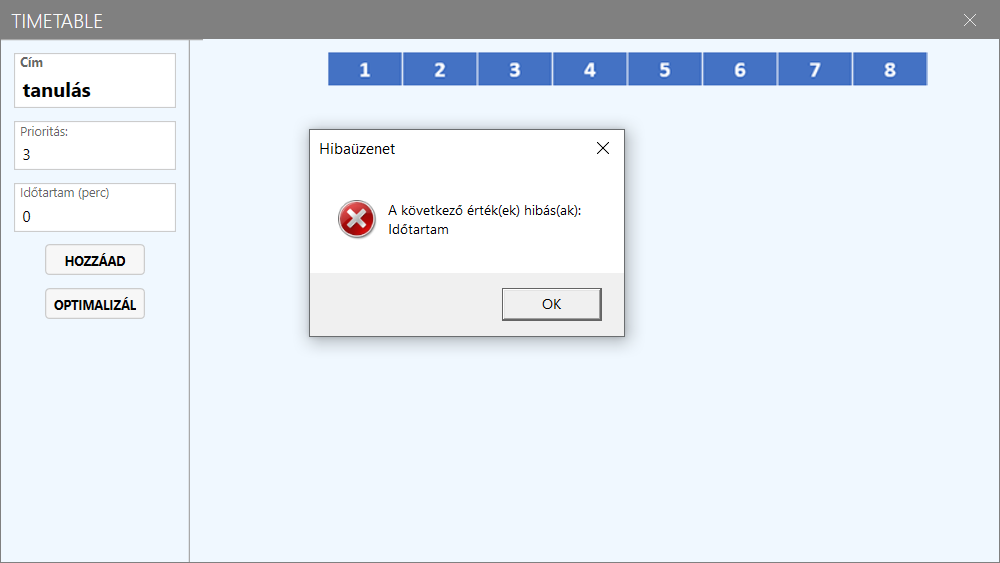
\includegraphics[width=\textwidth]{images/test/durationFault.png}
	\caption{Hibás adat megadása egy feladat hozzáada esetén}
	\label{fig:durationFault}
\end{figure}

A helyes kitöltés után egy felugró ablak jelezte a feladat sikeres hozzáadását, ezzel együtt a grafikus ábrázolás is megtörtént a diagramon.

A következő hibalehetőség felmerülése egy darab feladat optimalizálása során merülhet fel. Ilyenkor szintén hibaüzenet jelzi, hogy ennek a funkciónak az elvégzéséhez több feladat hozzáadására lenne szükség (\ref{fig:notEnoughTasks}. ábra).

\begin{figure}[h!]
	\centering
	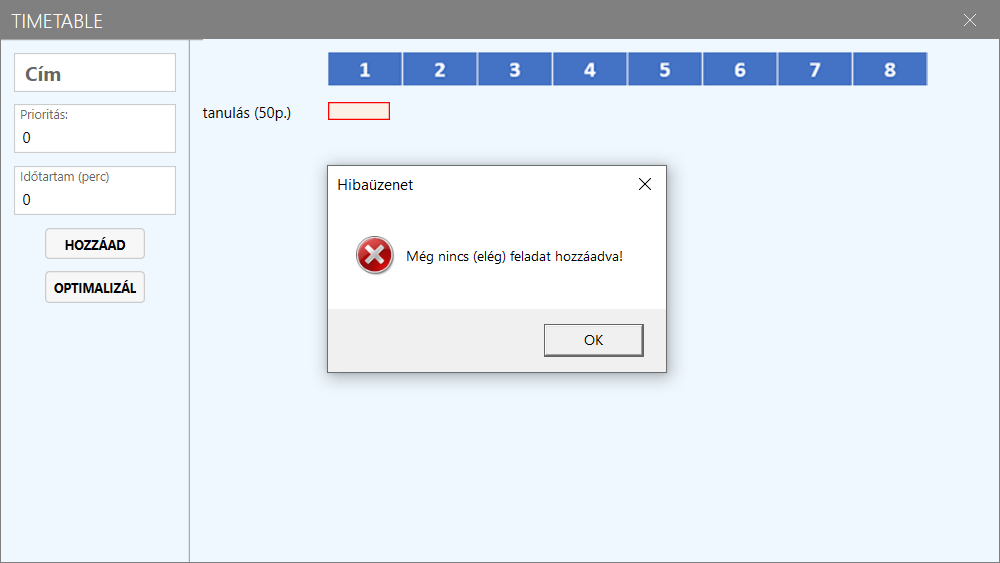
\includegraphics[width=\textwidth]{images/test/notEnoughTasks.png}
	\caption{Egy feladat esetén az ütemezés nem lehetséges}
	\label{fig:notEnoughTasks}
\end{figure}

A szemléltetés kedvéért ezek után hozzáadtam hosszabb és rövidebb tevékenységeket is, több különböző prioritással. 

\begin{figure}[h!]
	\centering
	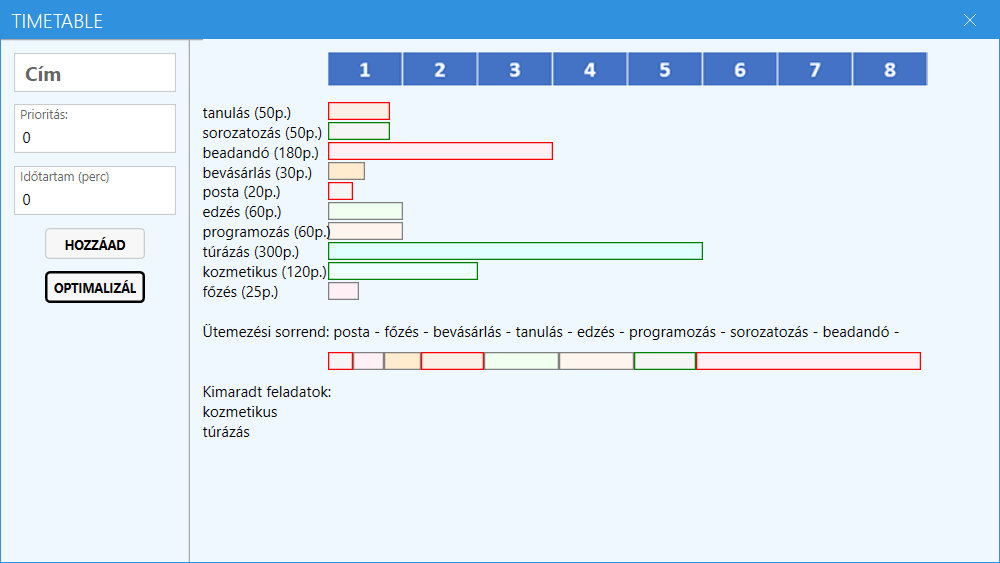
\includegraphics[width=\textwidth]{images/test/result1.png}
	\caption{Az 1. teszteset eredménye}
	\label{fig:result1}
\end{figure}

Végeredményben, mikor az optimalizálás és az ütemezés is lefutott, megjelent az előállított ütemterv, amely \aref{fig:result1}. ábrán látható. Megfigyelhető, hogy kettő feladat volt, ami már nem fért bele az ütemtervbe, mindkettő alacsony piroritással és hoszabb időtartammal rendelkezve. Ezeket a tevékenységeket külön jelzi is a program számunkra. A beütemezett feladatok közül pedig előre került egy magas prioritású feladat, követve azt egy közepes prioritásúval, amely rövid időtartama miatt is kerülhetett ennyire előre. Látható, hogy az ütemterv végén szintén magas prioritású feladat kapott helyet, ezt a többi feladathoz mérten hosszabb időtartamának köszönhette.

\Section{Teszteset 2.}

A második tesztesetben az előzőleg definiált tevékenységek újbóli megadása mellett, arra esett a választásom, hogy két feladat adatán módosítsak, megfigyelve, hogy a program az első tesztnél mennyivel különb eredményt ad. Az egyik a sorozatozás lett, amelynél ezúttal nem alacsony, hanem közepes prioritást választottam, az időtartamot meghagyva ugyanolyannak. A másik változás a beadandónál történt, itt a prioritást hagytam meg magas szinten, viszont az időtartamot jelentősen csökkentettem, az előző 3 óráról 30 percre. Így végeztem el az optimalizálást, ami \aref{fig:result1-2}. ábrán látható eredményt adta.

\begin{figure}[h!]
	\centering
	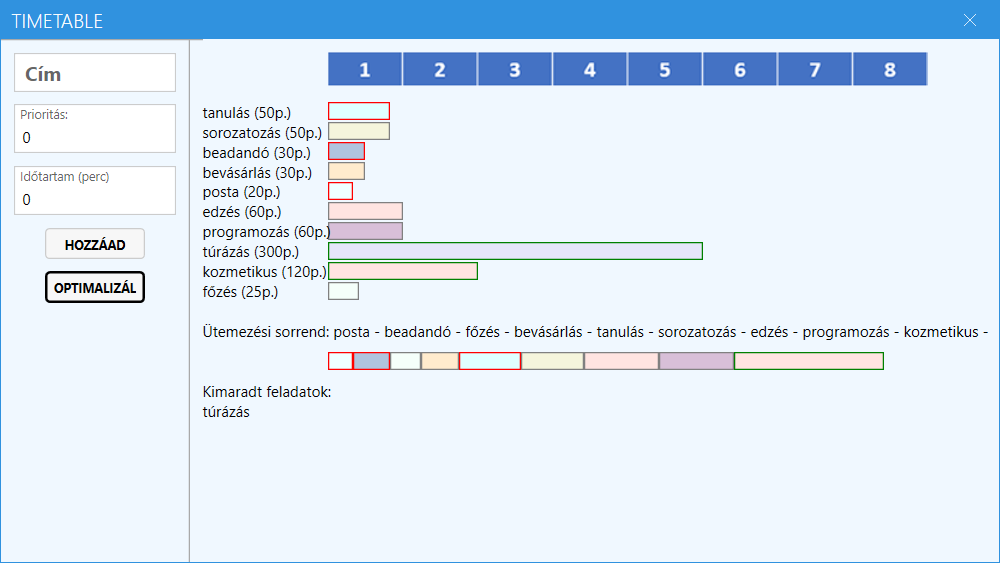
\includegraphics[width=\textwidth]{images/test/result1-2.png}
	\caption{Az 1. teszteset adatainak módosítása utáni eredmény}
	\label{fig:result1-2}
\end{figure}

Ami egyből feltűnhet az az, hogy az ütemtervből kimaradt feladatoknál már csak egy tevékenység szerepel, az előző kettőhöz képest. Ez evidens lehet, hiszen a beadandó időtartama jelentősen csökkent, így felszabadítva több helyet az időkeretben. A másik változás, hogy egyből két magas prioritású feladattal kezdődik az ütemterv, ebből a második az a beadandó írása, amely utolsó helyről került az elsők közé. A sorozatnézésnél is megfigyelhető a változás mértéke. A mostmár magasabb prioritásának köszönhetően, az ütemező hamarabbi időpontra ütemezte a sorban, megelőzve az edzés és a programozás tevékenységeket.

\Section{Teszteset 3.}

A harmadik példában már csak öt tevékenységet adtam meg, amelyek összideje 245 perc volt, azaz kicsit több, mint 4 óra. Az elvárt eredmény itt az volt, hogy ne maradjon ki feladat az ütemtervből, hiszen az időkeretbe belefér az összes feladat, de az ütemezett sorrendre nézve egy hatékony időbeosztás látszódjon. Ezt teljesítette is a program, a két magas prioritású tevékenységet ütemezte előre, kezdve a rövidebb időtartamúval. Ezt követően a közepes prioritású főzést megelőzte az alacsony prioritással rendelkező séta, köszönhetően annak, hogy arra fele annyi időt szántunk. Kimaradt feladatot nem jelzett a program (\ref{fig:result2}. ábra).

\begin{figure}[h]
	\centering
	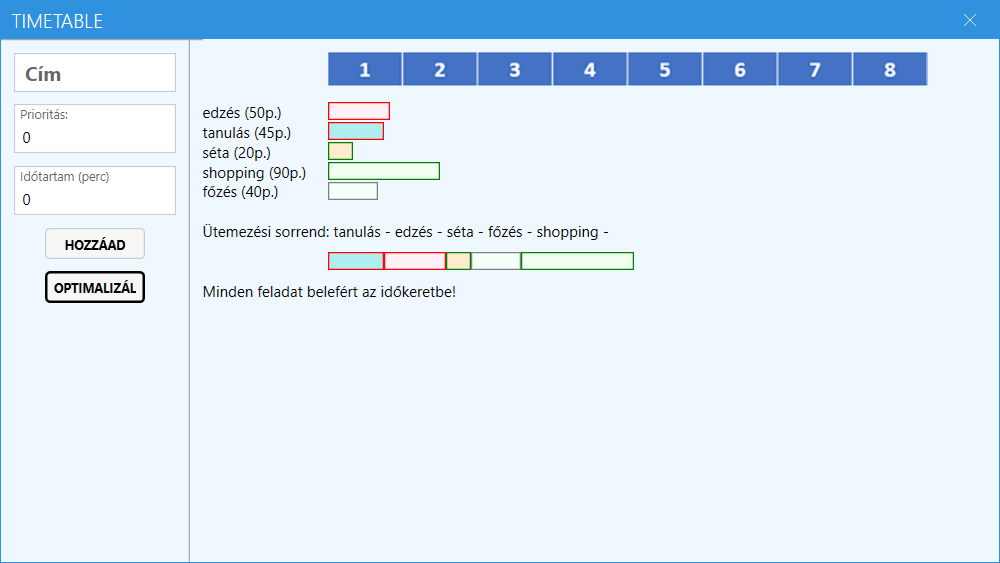
\includegraphics[width=\textwidth]{images/test/result2.png}
	\caption{Időkeretet túl nem haladó tevékenységek ütemezése}
	\label{fig:result2}
\end{figure}

\Section{Bővítési lehetőségek}

A szakdolgozatom olyan ütemezés és optimalizálás bemutatására szolgál, amely segít a mindennapi életben a teendők hatékony beütemezésében, ezáltal az időspórolásban, produktívabb életvitelben, mindezt diagramokon szemléltetve.

Az alkalmazásban még számtalan bővítési lehetőség van.
A továbbfejlesztés során lehetőség lenne például nem csak egy 8 órányi időkeretben történő ütemezésre, hanem akár heti szintű megvalósításra is. Továbbá, lehetne fix időpontban történő események megadását is lehetővé tenni, mint például egy fodrászat, fogászat vagy akár egy megbeszélt találkozó, hogy aztán az ütemező ezeket is figyelembe tudja venni.
Feladatok hozzáadásánál is számottevő bővítési lehetőség szóba jöhet, mint például:
\begin{itemize}
\item a prioritástartomány növelése,
\item színválasztás a grafikus megjelenítéshez,
\item több felhasználó hozzárendelése,
\item egyéb adatok (pl. feladat létrehozásának időpontjának) hozzárendelése,
\item helyadatok megadása,
\item sürgős feladatok jelölése a miharabbi beütemezéshez.
\end{itemize}
Mindemellett törlési funkció, heti összesítés, lekérdezések készítése is bővíthetné a program funkcionalitását.
